% VLDB template version of 2020-08-03 enhances the ACM template, version 1.7.0:
% https://www.acm.org/publications/proceedings-template
% The ACM Latex guide provides further information about the ACM template

\documentclass[sigconf, nonacm]{acmart}
\usepackage{mathtools}
\usepackage{xcolor}
\usepackage{amsfonts}
\usepackage{caption}
\usepackage{subfig}
\usepackage{changepage}
\usepackage{amsthm}

%% The following content must be adapted for the final version
% paper-specific
\newcommand\vldbdoi{XX.XX/XXX.XX}
\newcommand\vldbpages{XXX-XXX}
% issue-specific
\newcommand\vldbvolume{14}
\newcommand\vldbissue{1}
\newcommand\vldbyear{2020}
% should be fine as it is
\newcommand\vldbauthors{\authors}
\newcommand\ourmethod{Uniform UMAP}
\newcommand\vldbtitle{\shorttitle} 
% leave empty if no availability url should be set
\newcommand\vldbavailabilityurl{URL_TO_YOUR_ARTIFACTS}
% whether page numbers should be shown or not, use 'plain' for review versions, 'empty' for camera ready
\newcommand\vldbpagestyle{plain} 

\begin{document}
\title{A Thorough Analysis of and Improvement on UMAP and tSNE}

%%
%% The "author" command and its associated commands are used to define the authors and their affiliations.
\author{Andrew}
\author{Jakob}
\author{Katrine}
\affiliation{%
  \institution{Aarhus University}
  \streetaddress{Somewhere 5}
  \city{Aarhus}
  \state{}
  \postcode{8000}
  \country{}
}
\email{draganovandrew@cs.au.dk}
%%
%% The abstract is a short summary of the work to be presented in the
%% article.
\begin{abstract}
TSNE and UMAP have become two of the most popular dimensionality reduction algorithms due to their quick runtimes and intuitive low-dimensional embeddings.
Despite their ubiquity and similarities, however, there has not been a comprehensive attempt to fuse the two approaches into a single method. In this work, we
describe a general framework for comparing dimensionality reduction algorithms and analyze the differences between TSNE and UMAP in terms of this framework.
Under this framework, we identify which changes are necessary and sufficient to switch between the two approaches and disprove several claims regarding the
reason for each algorithms' efficacy, thus clarifying misconceptions regarding each algorithm.

Inspired by this, we create a new dimensionality reduction algorithm, \ourmethod, that combines the best characteristics of tSNE
and UMAP and is able to reproduce the results of either method with only a few hyperparameter changes. \ourmethod, when executed in a single thread, performs the optimization an order of magnitude faster than
multi-threaded UMAP and several orders of magnitude faster than multi-threaded tSNE on even modestly sized datasets. By virtue of its scalable characteristics,
we are able to effectively parallelize \ourmethod to obtain additional speed improvements. We also devise a new GPU
solution that performs our method's optimization significantly faster than existing GPU implementations of either UMAP or tSNE.

We lastly provide theoretical insights for future dimensionality reduction improvements. Our code is fully plug-and-play with the standard UMAP and tSNE
libraries and available to the public at \_\_\_\_.
\end{abstract}

\maketitle

%%% do not modify the following VLDB block %%
%%% VLDB block start %%%
\pagestyle{\vldbpagestyle}
\begingroup\small\noindent\raggedright\textbf{PVLDB Reference Format:}\\
\vldbauthors. \vldbtitle. PVLDB, \vldbvolume(\vldbissue): \vldbpages, \vldbyear.\\
\href{https://doi.org/\vldbdoi}{doi:\vldbdoi}
\endgroup
\begingroup
\renewcommand\thefootnote{}\footnote{\noindent
This work is licensed under the Creative Commons BY-NC-ND 4.0 International License. Visit \url{https://creativecommons.org/licenses/by-nc-nd/4.0/} to view a copy of this license. For any use beyond those covered by this license, obtain permission by emailing \href{mailto:info@vldb.org}{info@vldb.org}. Copyright is held by the owner/author(s). Publication rights licensed to the VLDB Endowment. \\
\raggedright Proceedings of the VLDB Endowment, Vol. \vldbvolume, No. \vldbissue\ %
ISSN 2150-8097. \\
\href{https://doi.org/\vldbdoi}{doi:\vldbdoi} \\
}\addtocounter{footnote}{-1}\endgroup
%%% VLDB block end %%%

%%% do not modify the following VLDB block %%
%%% VLDB block start %%%
\ifdefempty{\vldbavailabilityurl}{}{
\vspace{.3cm}
\begingroup\small\noindent\raggedright\textbf{PVLDB Artifact Availability:}\\
The source code, data, and/or other artifacts have been made available at \url{\vldbavailabilityurl}.
\endgroup
}
%%% VLDB block end %%%

\section{Introduction}
Dimensionality reduction (DR) algorithms are invaluable for qualitatively inspecting high-dimensional data and are used across computational and natural-science
disciplines for data visualization, denoising, graph embeddings, and many other tasks \textcolor{red}{REFERENCES}. Intuitively, DR algorithms accept a high-dimensional dataset as
input and find a faithful embedding in a lower-dimensional space. The term \textit{faithful} traditionally implies keeping similar points similar and dissimilar
points dissimilar, where similarity is measured by distance metrics or kernels in the corresponding spaces. This naturally implies a $O(n^2)$ runtime for many
nonlinear approaches, as we must compare the high- and low-dimensional pairwise distance matrices before we can be certain of the embedding quality.

Recent gradient-based methods have managed to improve on this by performing optimization only on relevant entries of the pairwise distance matrices.
Among these, TSNE and UMAP are by far the most popular due to their speed and intuitive results, each getting cited more than 1000 times per year on average.
They specifically overcome the $O(n^2)$ bound by constructing a setting in which distant points do not exert strong forces on one another, allowing the optimization to focus on nearest neighbors in the high dimensional space and sampling methods in the low-dimensional space.

Formally, TSNE \cite{van2008visualizing} and UMAP \cite{mcinnes2018umap} both receive an input dataset $X \in \mathbb{R}^{N \times D}$ of
$N$ points in $D$ dimensional space and
attempt to find a faithful embedding into a lower dimensional space $Y \in \mathbb{R}^{N \times d}$, where $d << D$. 
 In this paper, we refer to the pairwise squared distance matrices in high- and low-dimensional spaces as $E^X$ and $E^Y$, respectively.
Both algorithms model the problem as minimizing the KL divergence $\mathcal{L}(f(E^X), g(E^Y))$, where $f$ and $g$ are high- and
low-dimensional functions with respect to the distances. For both algorithms, $f$ is an inverse exponential function while $g$ is an inverse polynomial function --- chosen specifically to handle differences between high- and low-dimensional distance distributions.
We immediately see clear similarities between the two approaches; they share the same objective function structure, both optimize based
on sampling and nearest-neighbors and both utilize gradient descent to find the embedding. Despite their ubiquity and similarity, however, there has not been
a comprehensive attempt to unify the two methods.

In this paper, we first identify every framework choice and implementation discrepancy that differs between tSNE and UMAP. This allows us to describe each algorithm as a set of on/off
switches across the space of these differences. We then implement tSNE and UMAP in a common library, giving us the ability to study the effect of these
''switches`` on each of the algorithms.
We provide evidence that the most relevant changes are the choice of normalization on $E^X$ and $E^Y$ and the choice of gradient descent algorithm.
In fact, a majority of the differences between TSNE and UMAP turn out to be irrelevant in terms of both quantitative and qualitative analysis across datasets.
This refutes several claims made in both the TSNE and UMAP papers regarding the necessary components of their approaches.

Based on this analysis we propose \ourmethod, an embedding algorithm that recreates both tSNE and UMAP embeddings by changing just two input parameters.
We experimentally validate that \ourmethod can simulate both methods through quantitative metrics and qualitative
evaluations. Surprisingly, we also show that the choice of optimizing the KL divergence is not set in stone, finding that minimizing the Frobenius norm provides
embeddings of a similar quality despite significantly simpler gradient calculations. Due to these improvements, \ourmethod is particularly amenable to
parallelization, recreating UMAP's embeddings 5-times faster and TSNE's several orders of magnitude faster.
Lastly, our library includes the option for GPU code, giving us the fastest method for optimizing TSNE and UMAP embeddings in any algorithm/processor setting.
Our code is fully compatible with each algorithm's current popular implementation and available at \_\_\_\_.

In summary, our contributions are as follows:
\begin{enumerate}
        \item We perform the first full analysis of every difference between the TSNE and UMAP algorithms, identifying which changes are necessary to
        convert one algorithm to the other.
        \item We propose \ourmethod, an optimization algorithm that effectively recreates either TSNE or UMAP embeddings as dictated by only two input
            parameters.
        \item We release a simple, plug-and-play implementation of our approach, providing significant speed improvements for TSNE and UMAP on both
        the CPU and GPU.
\end{enumerate}

\section{Related Work}

\ourmethod falls into a broad category of gradient based DR approaches, characterized by minimizing a non-convex objective using variants of gradient descent.
We have already presented TSNE and UMAP, which are the two most common, but there exist several variations on each of these algorithms. When discussing TSNE, we
refer to \cite{van2014accelerating}, which established the nearest neighbor and sampling speed improvements. Since this paper, a popular subsequent improvement
was presented in \cite{linderman2019fast}, wherein Fast Fourier Transforms were used to accelerate the comparisons between points. Another approach based on
TSNE is the LargeVis algorithm, proposed in \cite{tang2016visualizing}, which modifies the embedding functions to satisfy a Bernoulli probabilistic model of
the low-dimensional dataset. As the more recent algorithm, UMAP has not had as many variations yet. One promising direction, however, has been to extend the
second step of UMAP as a parametric optimization on neural network weights \cite{sainburg2020parametric}.

There have been several papers that attempt to explain the difference between TSNE and UMAP. In both \cite{kobak2019umap} and \cite{kobak2021initialization},
the argument is made that the necessary and sufficient condition to switch between their embeddings is the difference in initialization between the two methods.
Namely, TSNE randomlyinitializes the low-dimensional dataset whereas UMAP first calculates a Laplacian Eigenmap \cite{belkin2003laplacian} embedding before
beginning the optimization. We have been unable to reproduce these results across datasets and optimization criteria, a topic we discuss later in our results.

Lastly, we also mention the state-of-the-art implementations of both TSNE and UMAP on the GPU. The CPU implementations are found in the scikit-learn and
umap-learn python libraries for TSNE and UMAP, respectively. The fastest current implementations on the GPU, however, can be found in the RAPIDS AI
framework \cite{nolet2020bringing} \cite{rapidsframework}.

\section{Comparison of tSNE and UMAP} \label{comparison}
We begin by formally introducing the tSNE and UMAP DR algorithms. Let $X \in \mathbb{R}^{N \times D}$ be the high dimensional dataset of $N$ points and let $Y
\in \mathbb{R}^{N \times d}$ be a previously initialized set of $N$ points in lower-dimensional space such that $d << D$. 

We now respectively establish Gaussian and student-t kernels on the high- and low-dimensional distances to represent the likelihood that $x_i$ and $y_i$ choose
$x_j$ and $y_j$ as their respective nearest neighbors. These kernels are defined by
\begin{align}
    % FIXME - the denominator here isn't quite right
    p^{tsne}_{j|i}(x_i, x_j) &= \dfrac{\text{exp}(-d(x_i, x_j)^2 / 2 \sigma_i^2)}{\sum_{k \neq l} \text{exp}(-d(x_k, x_l)^2 / 2 \sigma_k^2)} \\[0.5ex]
    q^{tsne}_{ij}(y_i, y_j) &= \dfrac{(1 + ||y_i - y_j||^2_2)^{-1}}{\sum_{k \neq l} (1 + ||y_k - y_l||^2_2)^{-1}} \\[1.5ex]
    p^{umap}_{j|i}(x_i, x_j) &= \dfrac{\text{exp} (-d(x_i, x_j)^2 + \rho_{i})}{\tau_i} \\[0.3ex]
    q^{umap}_{ij}(y_i, y_j) &= \left( 1 + a(||y_i - y_j||^2_2)^b \right) ^{-1}
\end{align}
where $d(x_i, x_j)$ is the high-dimensional distance function, $\sigma$ and $\tau$ are point-specific variance scalars, $\rho_i = \min_{j \neq i} d(x_i, x_j)$,
and $a$ and $b$ are constants. In practice, we can assume that $2 \sigma_i^2$ is functionally equivalent to $\tau_i$, and we will use $\tau$ when referring to
this kernel variance term. The high-dimensional kernels are symmetrized by applying symmetrization functions. Without loss of generality, let $p_{ij}
= S(p_{j|i}, p_{i|j})$ for some symmetrization function $S$.

The principal difference in these functions is the normalization factor. tSNE scales the high- and low-dimensional kernels by all of the pairwise
relationships whereas UMAP allows the Gaussian and Student-t kernels to remain untouched\footnote{We note that the tSNE papers give the impression that
high-dimensional normalization 
occurs across rows, while in reality the code performs normalization across the entire pairwise kernel matrix.}. This implies a different probabilistic
interpretation between the two algorithms. In the case of tSNE, the weights are normalized across the entire matrix of pairwise relations, giving us 
a probability distribution across the entire dataset. In the case of UMAP, our pairwise kernels remain unnormalized, implying a Bernoulli distribution along
each edge that can be interpreted as the likelihood of that edge existing.

Each algorithm then applies gradient descent with respect to the KL-divergence(s) between these probability distributions. We refer to the high- and
low-dimensional pairwise kernel matrices as $P = \left( p_{ij} \right)_{i, j < N}$ and $Q = \left( q_{ij}
\right)_{i, j < N}$ respectively. This gives us the loss functions
\begin{align}
    \mathcal{L}_{tsne} &= \text{KL} (P || Q) = \sum_{i \neq j} p_{ij} \log \dfrac{p_{ij}}{q_{ij}} \\
    \mathcal{L}_{umap} &= \sum_{i \neq j} \left[ p_{ij} \log \dfrac{p_{ij}}{q_{ij}} + (1 - p_{ij}) \log \dfrac{1 - p_{ij}}{1 - q_{ij}} \right]
\end{align}
In essence, tSNE minimizes the KL divergence of the entire pairwise kernel matrices whereas UMAP sums over each edge's KL divergence in terms of the Bernoulli distribution.

\subsection{Intuition}

We would like to provide some intuition for these two normalizations. In the normalized case we have a probability distribution over all
distinct pairwise relationships $p(x_i, x_j)$ and $q(y_i, y_j)$ for $i \neq j$. In the unnormalized case we instead have a probability distribution over each
individual distinct pairwise relationship. We can look at these through the lens of a fully-connected graphs in which each edge $e_{ij}$ is the
kernel value $p(x_i, x_j)$ or $q(y_i, y_j)$. Under this lens, the probabilities in the normalized case are akin to asking ``when we pick a random edge, what is the
probability that we pick $e_{ij}$?''. Alternatively, the unnormalized variant asks ``for the specific edge $e_{ij}$, what is the probability that it exists?''
Minimizing the KL divergence therefore amounts to ensuring that these probabilities in the high- and low-dimensional spaces are as similar as possible.

In practice, both tSNE and UMAP optimize this KL divergence by separately calculating attractive and repulsive forces. It is unnecessary to calculate
every single attraction and repulsion though, as dissimilar points in the high-dimensional space impose negligible attraction in the low-dimensional space.
To simplify the complexity, both approaches establish a nearest neighbor graph \cite{van2014accelerating} with edges $|\mathcal{E}|$ among the
high-dimensional points where points $x_i$ and $x_j$ share an edge if either $x_i$ is $x_j$'s nearest neighbor or $x_j$ is $x_i$'s nearest neighbor.
Then both algorithms simply perform attractions along these edges while performing repulsions evenly across the rest of the points. In this sense, we can
interpret the gradient descent problem as a set of springs between every pair of points in $Y$ where the spring constants are determined by the Gaussian and
Student-t kernels.

\subsection{Gradients}

The gradients of each algorithm change substantially due to the differing normalizations. In tSNE, the gradient can be written as
\begin{equation}
    \dfrac{\partial \mathcal{L}_{tsne}}{\partial y_i} = 4 \sum_{j \neq i} (p_{ij} - q_{ij}) q_{ij} Z (y_i - y_j)
\end{equation}
where $Z = \sum_{k \neq l} (1 + ||y_k - y_l||_2^2)^{-1}$ is the normalization factor for the low-dimensional kernel. This is often represented as an attractive
and repulsive force with
\begin{align*}
    \dfrac{\partial \mathcal{L}_{tsne}}{\partial y_i} &= 4(\mathcal{A}_i^{tsne} + \mathcal{R}_i^{tsne}) = \\
    &= 4 \left[ - \sum_{j, j \neq i} p_{ij}q_{ij}Z (y_i - y_j) + \sum_{j, j \neq i} q_{ij}^2 Z (y_i - y_j) \right]
\end{align*}

UMAP also describes separating its gradient into attractive and repulsive terms\footnote{$p_{ij}$ are the calculated nearest neighbor weights in the
high-dimensional space. $p_{ik}$, on the other hand, are the potentially unknown pairwise weights between point $i$ and a randomly selected point $k$}, with
\begin{align}
    \mathcal{A}_i^{umap} = & \sum_{j, j \neq i} \dfrac{-2ab||y_i - y_j||_2^{2(b-1)}}{1 + ||y_i - y_j||_2^2} p_{ij} (y_i - y_j) \label{umap_attr} \\
    \mathcal{R}_i^{umap} = & \sum_{j, j \neq i} \dfrac{2b}{(\epsilon + ||y_i - y_k||_2^2)(1 + a ||y_i - y_k||_2^{2b})} \cdot \label{umap_rep} \\
    &\cdot (1 - p_{ik}) (y_i - y_k) \nonumber
\end{align}

We make the argument that this change in normalization is the fundamental difference between the two algorithms. First, note that the UMAP repulsive force is
inversely quadratic with respect to the low-dimensional distance. This means that points that are too close in the low-dimensional space experience
significantly stronger repulsions under UMAP's gradients than under TSNE's. This can be seen in figures \ref{fig:linear_grads} and \ref{fig:exp_grads}, where we
plot the force between points $y_i$ and $y_j$ as a function of their high- and low-dimensional distances.
Additionally, the normalization has a direct effect on the accumulated gradient force during a single epoch.
By not normalizing, UMAP's pairwise likelihoods have orders of magnitude $p_{ij}, q_{ij} ~ 0.5$, whereas TSNE's are bounded by the fact that $\sum_{i \neq j}
p_{ij} = \sum_{i \neq j} q_{ij} = 1$.
This means that the average TSNE spring force is significantly weaker than the average UMAP one.
However, TSNE and UMAP calculate comparable numbers of attractions and repulsions during every epoch, naturally leading to UMAP collecting significantly
stronger per-point gradients over the span of an epoch of gradient descent.


\begin{figure}
\centering
	\subfloat[\centering tSNE gradients]{{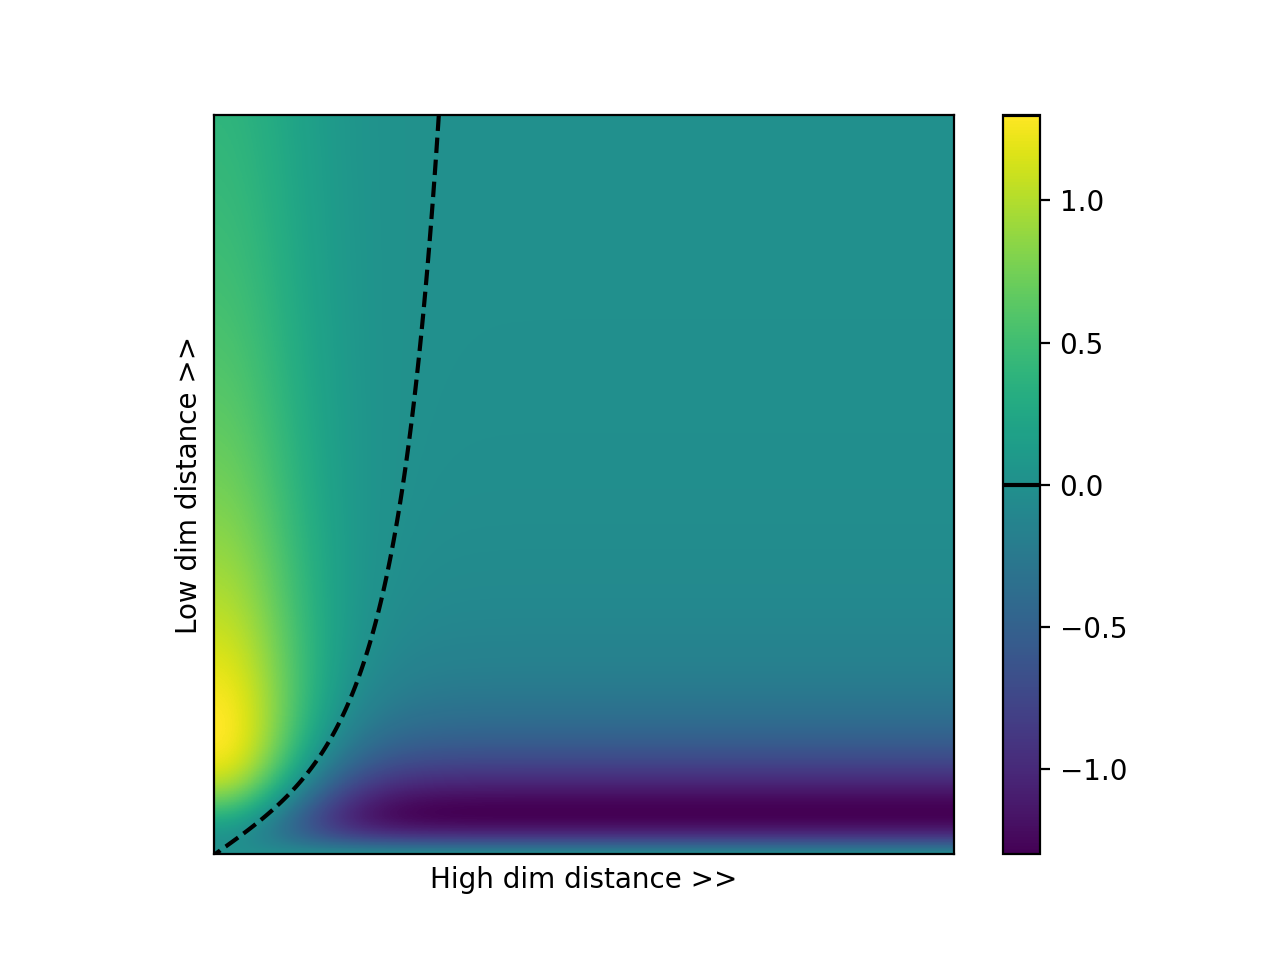
\includegraphics[width=7cm]{tex_images/tsne_grad.png} }}%
	\qquad
	\subfloat[\centering UMAP gradients]{{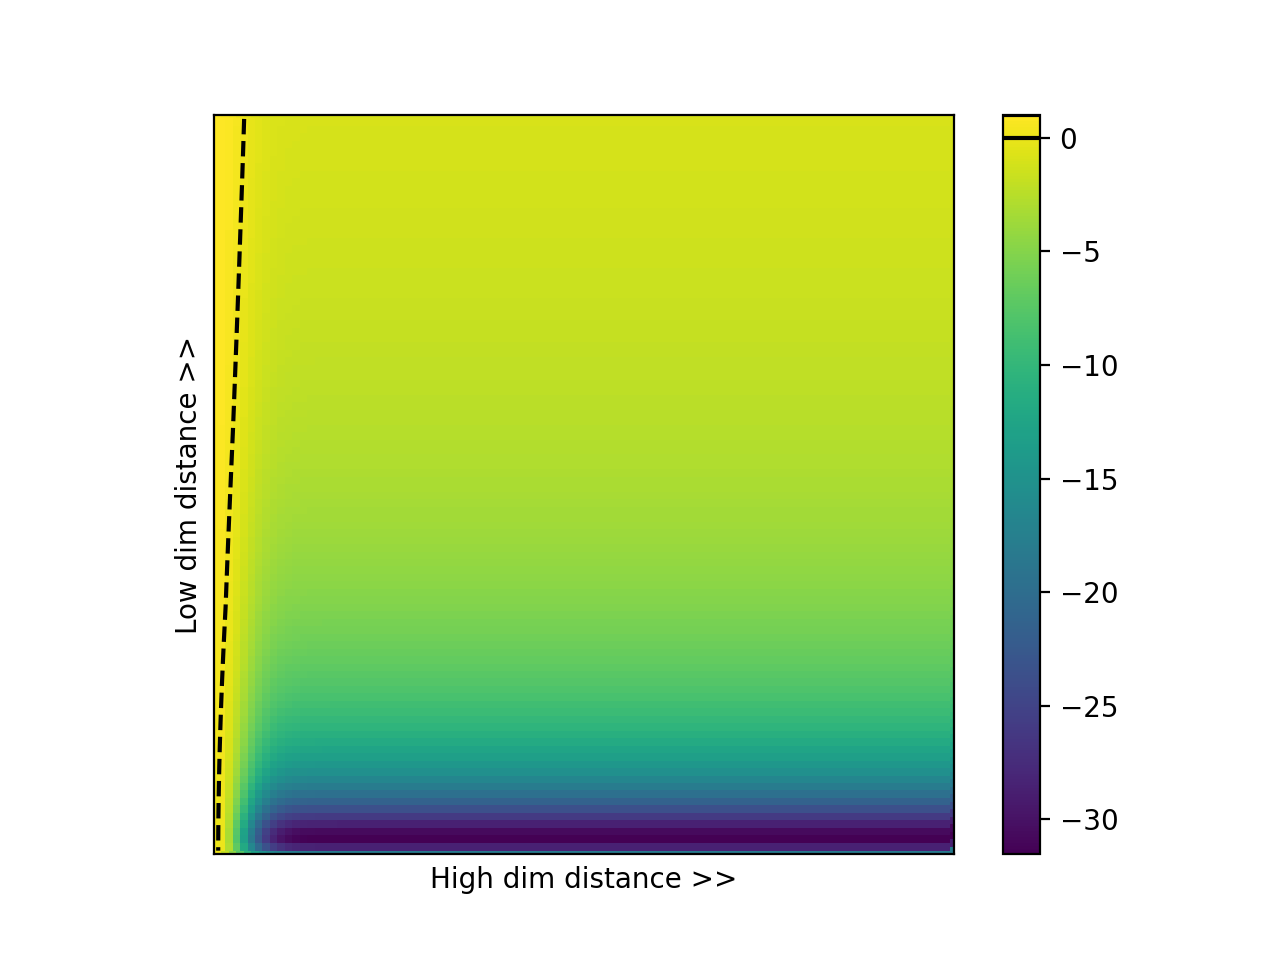
\includegraphics[width=7cm]{tex_images/umap_grad.png} }}%
	\caption{A comparison of tSNE and UMAP gradients for linearly growing distances}%
	\label{fig:linear_grads}%
\end{figure}

\begin{figure}
\centering
	\subfloat[\centering tSNE gradients]{{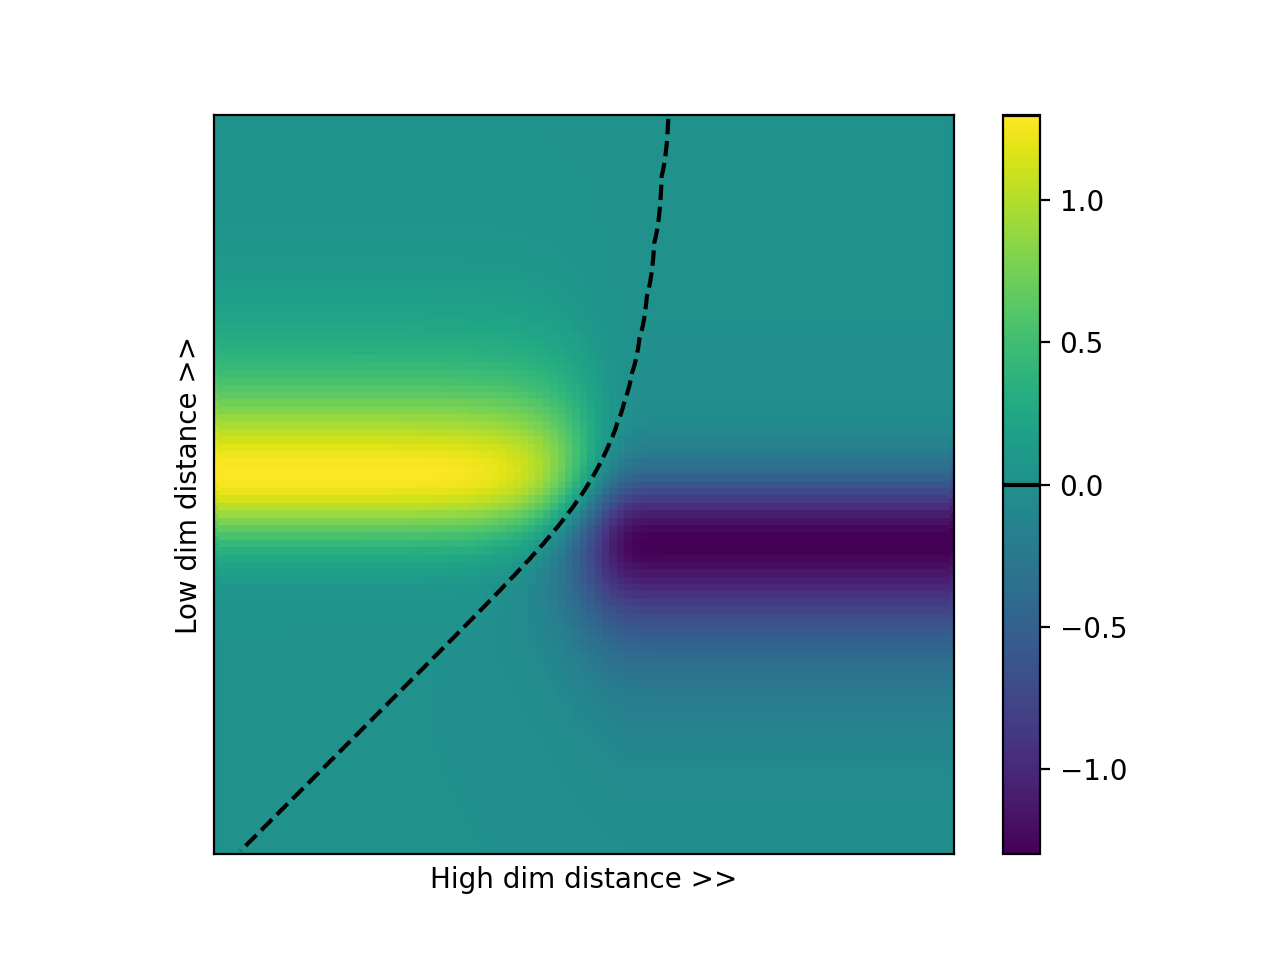
\includegraphics[width=7cm]{tex_images/tsne_exp_grads.png} }}%
	\qquad
	\subfloat[\centering UMAP gradients]{{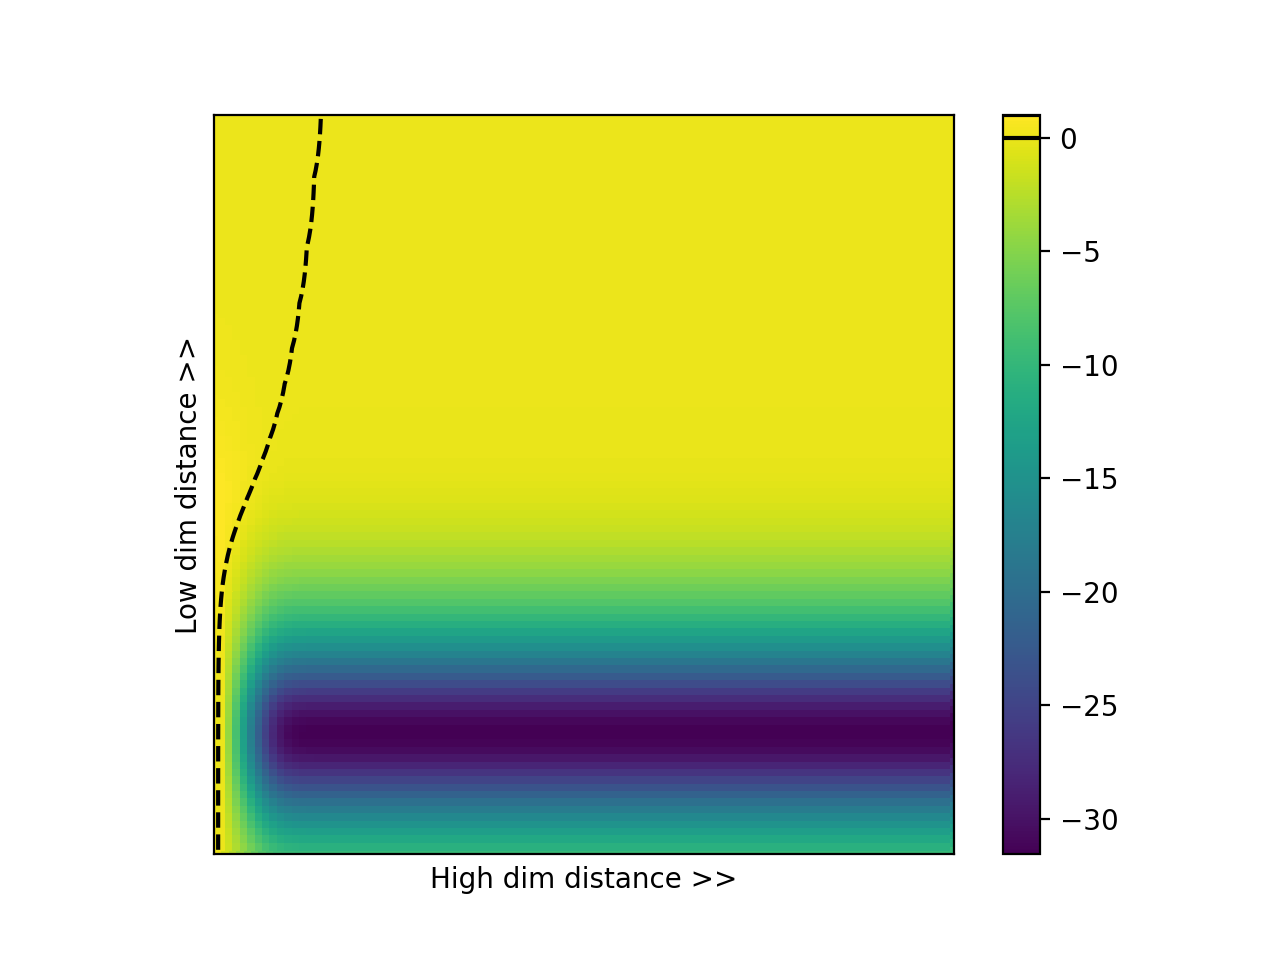
\includegraphics[width=7cm]{tex_images/umap_exp_grads.png} }}%
	\caption{A comparison of tSNE and UMAP gradients for exponentially growing distances}%
	\label{fig:exp_grads}%
\end{figure}

\subsection{Implementation differences} \label{implementation_diffs}
Given the above descriptions of the algorithms, we now describe every implementation difference between them. Section \ref{results} will discuss the
practical effect that each of these has on the results.

\begin{itemize}
    \item Gradient Descent
        \begin{itemize}
        \item TSNE collects all of the attractive and repulsive forces before applying momentum gradient descent across every point.
            \begin{itemize}
            \item tSNE's gradient descent has an additional scalar that amplifies the force if a point moves in the same direction at time $t+1$ as it did at time $t$
                and dampens the force otherwise.
            \end{itemize}
        \item In contrast, UMAP updates the position of every point immediately upon calculating the attractive and repulsive forces acting on it.
        \end{itemize}

    \item Scalars
        \begin{itemize}
        \item UMAP uses scalars $a$ and $b$ to manage the distribution of $Q$.
        \item TSNE operates under the assumption that $a = b = 1$.
        \end{itemize}

    \item Attractive Force Sampling
        \begin{itemize}
        \item TSNE applies every attractive force at every epoch.
        \item UMAP simulates the $p_{ij}$ scalar in \ref{umap_attr} by only applying the force every $1 / p_{ij}$ epochs.
            \begin{itemize}
                \item We note that UMAP similarly scales the repulsive forces by sampling them at a rate of $1 / (1 - p_{ik}$
            \end{itemize}
        \end{itemize}

    \item Repulsive Force Sampling
        \begin{itemize}
        \item TSNE estimates each point's repulsion from every other point using Barnes-Hut trees.
        \item UMAP only calculates repulsive forces with respect to $k$ randomly sampled points.
        \end{itemize}

    \item Force Application
        \begin{itemize}
        \item UMAP applies the attractive force between $y_i$ and $y_j$ to both $y_i$'s and $y_j$'s positions
        \item tSNE applies the attractive force to only $y_i$.
        \end{itemize}
        We refer to these options as \textit{symmetric} and \textit{asymmetric} attraction.

    \item Nearest Neighbors
        \begin{itemize}
        \item tSNE takes the time to identify exact nearest neighbor relationships.
        \item UMAP finds approximate nearest neighbors using nearest-neighbor descent \cite{dong2011efficient}.
        \end{itemize}

    \item Distance Calculations
        \begin{itemize}
        \item UMAP's high dimensional kernel on points $x_i$ and $x_j$ subtracts the minimum squared distance $\rho_i = \min_{k \neq i} d(x_i, x_k)^2$. The theoretical
        justification for this is discussed at length in the UMAP paper. 
        \item TSNE uses the traditional squared distance metric.
        \end{itemize}

    \item Symmetrization
        \begin{itemize}
        \item tSNE symmetrizes the high-dimensional kernels with $S_{tsne}(p_{j|i}, p_{i|j}) = (p_{j|i} + p_{i|j}) / 2$.
        \item UMAP uses a probabilistic symmetrization with $S_{umap}(p_{j|i}, p_{i|j}) = p_{j|i} + p_{i|j} - p_{j|i} \cdot p_{i|j}$.
        \end{itemize}

    \item Initialization
        \begin{itemize}
        \item tSNE randomly initializes $Y$.
        \item UMAP initializes with a Laplacian Eigenmap projection.
        \end{itemize}

\end{itemize}

\subsection{Comparison Implementation}
In order to evaluate each of the above changes, we re-implemented the TSNE and UMAP algorithms such that each choice can be freely applied onto both algorithms.
There are a few complications that we would like to mention, however. The fact that UMAP applies gradients live inside the optimization loop is incompatible
with momentum gradient descent or the change in normalization. This is due to the fact that the forces under normalization or momentum gradient
descent rely on scalars that are gathered over the course of the entire epoch. As such, both of these were evaluated on a variant of UMAP in which gradients are
collected across the epoch before being applied. We find that collecting gradients vs. applying them immediately does not change the resulting
embedding in any of our experiments.

\section{\ourmethod} \label{uniform}
We now present \ourmethod  --- an algorithm that can recreate both TSNE and UMAP results at much higher speeds than any implementation of either algorithm.
The key observation is noticing that the only two necessary ''switches`` are the normalization and the usage of momentum during the gradient descent. In fact,
every other discrepancy between the algorithm is inconsequential across datasets and domains. This allows us to remove TSNE's reliance on the costly Barnes-Hut
trees and instead perform repulsions due to sampling.
Furthermore, by removing UMAP's reliance on sampling to simulate $p_{ij}$ and $1 - p_{ik}$, we also remove the need for performing multiple repulsions for every
attraction.\footnote{We note that not most values of $p_{ik}$ are unavailable to us during optimization. We overcome this by setting $p_{ik} = 1 - \bar{p}_{ij}
\; \forall \; p_{ik}$. UMAP's implementation similarly does not calculate $p_{ik}$, instead using $p_{ik} \approx p_{ij}$ as an estimation.} We exprimentally
validate that these changes still allow us to obtain both TSNE's and UMAP's embeddings despite the significantly simplified optimization loop.

With respect to the other choices, \ourmethod  uses TSNE's asymmetric attraction, distance-metric, and gradient collection along with UMAP's
initialization, scalars, nearest neighbors, and symmetrization.

We also point out the curious fact that optimizing the KL divergence is not a necessary condition to achieve compelling embeddings. Indeed, we find that one can
instead optimize the Frobenius norm without sacrificing quality:
\[ \mathcal{L}(X, Y) = \sum_{i \neq j} (p(x_i, x_j) - q(y_i, y_j))^2 \]

This presents us with the following attractive and repulsive forces acting on point $y_i$
% FIXME -- check these to be totally correct
\begin{align*}
    \mathcal{A}_i^{frob-tsne} &= -4ab \sum_{j, j \neq i} p_{ij} Z (q_{ij}^2 + 2q_{ij}^3) (y_i - y_j) \\
    \mathcal{R}_i^{frob-tsne} &= 4ab \sum_{j, j \neq i} Z( q_{ij}^3 + 2q_{ij}^4) (y_i - y_j) \\
    &\\
    \mathcal{A}_i^{frob-umap} &= -4ab \sum_{j, j \neq i} p_{ij} q_{ij}^2 (y_i - y_j) \\
    \mathcal{R}_i^{frob-umap} &= 4ab \sum_{j, j \neq i} q_{ij}^3 (y_i - y_j)  
\end{align*}

Although this does not necessarily simplify the TSNE calculations, the UMAP gradients are significantly cleaner as we have reduced the number of non-integer
power relationships and removed the need for estimating $1 - p_{ik}$. We find that the resulting embeddings are also more consistent.

% \section{Embedding Results} \label{results}
% We now show that, subject to the change in \ref{uniform}, one can directly implement both tSNE and UMAP through either framework. We first show that Uniform UMAP
% can successfully recreate UMAP's outputs across a variety of datasets. Then, we go through the elements in \ref{implementation_diffs} to identify what effect
% each choice has on the tSNE and Uniform UMAP embeddings. Using this, we identify the changes necessary to produce tSNE's outputs within the UMAP framework and vice versa.
% 
% \subsection{Metrics}
% To avoid relying on qualitative observation, we introduce several metrics that we will be using to describe both embedding quality and the differences between tSNE and UMAP.
% 
% Want one metric that is ``quality of embedding'' and one that captures ``amount of space between clusters''. For the latter, it should be enough to get
% distances of all points between two clusters and take the 1\% cut. Basically, something to give you the distance between the shells of the two clusters.
% % \begin{enumerate}
% %     \item Change in sort index - If we sort the high-dimensional distances and the low-dimensional distances, how different are the sort indices? The x-axis
% %         goes through all the high-dimensional distances in order; the y-axis is the relative change for that high-dimensional sort index
% %     \item High dimensional distance vs. low dimensional distance - These are simply the low-dimensional distances plotted vs. the high dimensional distances. The high dimensional distances
% %         have been sorted from least to greatest. Note that PCA is a straight line (which is what we expected). Also, note that the large high-dim distances are
% %         represented by larger low-dim distances in UMAP than in tSNE
% %     \item Sorted distances - This is just the y-values of the previous plot. Basically, when we sort the high-dimensional distances, what do the low
% %         dimensional ones look like?
% %     \item Nearest neighbor overlap - For every point, what percent of its [k, k + 10] nearest neighbors are preserved? Note that immediate local distances are preserved in
% %         tSNE and UMAP, after which there is a giant portion where the middle distances aren't relevant.
% %     \item Relative error - This is the relative error for high-dimensional distances. We normalize both the high-dim and low-dim distances to $[0, 1]$, since the
% %         magnitudes are arbitrary in our setting. Thus, we do $| (d^h(x_i, x_j) - d^l(y_i - y_j)) |/ d^h(x_i, x_j)$. We replace the 0's in the high dimensional
% %         distances with 1's to avoid division errors.
% % \end{enumerate}
% 
% \subsection{UMAP and Uniform UMAP Equivalency}
% 
% \subsection{Analysis of Implementation Choices}
% 
% \subsection{Achieving tSNE within UMAP}
% The main obstacle to overcome is undoing the normalization
% differences between tSNE and UMAP. In fact, tSNE can be achieved within the UMAP implementation through the following modifications:
% \begin{enumerate}
%     \item Normalize the high- and low-dimensional kernels as they are normalized in tSNE
%     \item Perform tSNE's gradient descent as described in \ref{uniform}
%     \item Apply asymmetric attraction forces
% \end{enumerate}
% Due to using tSNE's normalization, we also require the corresponding modification to the KL divergence. As such, we obtain gradients
% \begin{align*}
%     F_{attr} &= 4 \sum_{j \neq i} p_{ij} q_{ij} Z (y_i - y_j) \\
%    F_{rep} &= 4 \sum_{j \neq i} q_{ij}^2 Z (y_i - y_j)
% \end{align*}
%    where
% \begin{align*}
%    q_{ij} &= \dfrac{(1 + a ||y_i - y_j||_2^{2b})^{-1}}{\sum_{k \neq l} (1 + a ||y_i - y_j||_2^{2b})^{-1}} \\
%     p_{j|i} &= \dfrac{\text{exp}( -(d(x_i, x_j)^2 - \rho_i) / \tau_i)}{\sum_{k \neq l} \text{exp}( (-d(x_k, x_l)^2 + \rho_i) / \tau_k)}
% \end{align*}
%    and $Z = \sum_{k \neq l} (1 + a ||y_i
%    - y_j||_2^{2b})^{-1}$. Notice that this is essentially the tSNE kernels with UMAP's $\rho_i$, $a$, and $b$ scalars. We show later that these can be removed
%    in practice.
% 
% \subsection{Achieving UMAP within tSNE}
% This direction turns out to be significantly easier. Performing the Barnes-Hut algorithm for tSNE with a Laplacian eigenmap initialization and symmetric
% attraction is sufficient to obtain UMAP consistently.
% 
% \subsection{Claims and misconceptions}
% % FIXME - talk about GAINS in tSNE optimization
% We would like to discuss several claims regarding these algorithms' choices and use-cases. Firstly, we'd like to note that the tSNE paper mentions
% that the high-dimensional probabilities $p_{j|i}$ are normalized by the sum $\sum_{k \neq i} \exp\left( ||y_i - y_k||^2 \right) / \tau_i$. To the authors of
% this paper and other people whom we've spoken to, this implies that the normalization occurs across rows of the pairwise probability matrix. Instead, tSNE
% implementations normalize $p_{j|i}$ across the entire pairwise probability matrix, giving us symmetric normalizations in the high- and low-dimensional spaces (a
% necessary condition for the KL divergence).
% 
% Additionally, there are several choices made in UMAP that do not provide practical changes. Namely, we find that the choice of normalization is the
% single necessary condition for switching between tSNE and UMAP.
% This puts the practical necessity of multiple components of UMAP's algorithm into question. The first of these is the pseudo-distance metric $\tilde{d}_i(x_j, x_k) = ||x_j - x_k||_2^2
% - \rho_i$. Its inclusion theoretically justifies that the nearest-neighbor graph captures the topology of the high-dimensional dataset. Despite the sound
% theoretical derivations we find across datasets, metrics, and contexts that subtracting the minimum distance has a negligible effect on the resulting
% embeddings. We also refute the assertion that tSNE's lack of a mathematical framework prohibits it from being
% extended; specific examples include embedding unseen
% points given an existing projection, utilizing categorical variables, and consolidating differing metrics. Our implementation of Uniform UMAP is able
% to, under tSNE's normalization and optimization schema, perform all of these tasks in the same manner as UMAP while obtaining results in line with tSNE's. Lastly, there have been claims made that tSNE
% with the Laplacian eigenmap initialization recreates UMAP's outputs \cite{kobak2019umap} or that the initialization is primarily responsible for the quality of
% the resulting embedding \cite{kobak2021initialization}. While this may be true for certain datasets, we do not observe it to be the case universally.


\bibliographystyle{ACM-Reference-Format}
\bibliography{references}

\end{document}
\endinput
